% Options for packages loaded elsewhere
\PassOptionsToPackage{unicode}{hyperref}
\PassOptionsToPackage{hyphens}{url}
\PassOptionsToPackage{dvipsnames,svgnames,x11names}{xcolor}
%
\documentclass[
  letterpaper,
  DIV=11,
  numbers=noendperiod]{scrartcl}

\usepackage{amsmath,amssymb}
\usepackage{iftex}
\ifPDFTeX
  \usepackage[T1]{fontenc}
  \usepackage[utf8]{inputenc}
  \usepackage{textcomp} % provide euro and other symbols
\else % if luatex or xetex
  \usepackage{unicode-math}
  \defaultfontfeatures{Scale=MatchLowercase}
  \defaultfontfeatures[\rmfamily]{Ligatures=TeX,Scale=1}
\fi
\usepackage{lmodern}
\ifPDFTeX\else  
    % xetex/luatex font selection
\fi
% Use upquote if available, for straight quotes in verbatim environments
\IfFileExists{upquote.sty}{\usepackage{upquote}}{}
\IfFileExists{microtype.sty}{% use microtype if available
  \usepackage[]{microtype}
  \UseMicrotypeSet[protrusion]{basicmath} % disable protrusion for tt fonts
}{}
\makeatletter
\@ifundefined{KOMAClassName}{% if non-KOMA class
  \IfFileExists{parskip.sty}{%
    \usepackage{parskip}
  }{% else
    \setlength{\parindent}{0pt}
    \setlength{\parskip}{6pt plus 2pt minus 1pt}}
}{% if KOMA class
  \KOMAoptions{parskip=half}}
\makeatother
\usepackage{xcolor}
\setlength{\emergencystretch}{3em} % prevent overfull lines
\setcounter{secnumdepth}{5}
% Make \paragraph and \subparagraph free-standing
\ifx\paragraph\undefined\else
  \let\oldparagraph\paragraph
  \renewcommand{\paragraph}[1]{\oldparagraph{#1}\mbox{}}
\fi
\ifx\subparagraph\undefined\else
  \let\oldsubparagraph\subparagraph
  \renewcommand{\subparagraph}[1]{\oldsubparagraph{#1}\mbox{}}
\fi

\usepackage{color}
\usepackage{fancyvrb}
\newcommand{\VerbBar}{|}
\newcommand{\VERB}{\Verb[commandchars=\\\{\}]}
\DefineVerbatimEnvironment{Highlighting}{Verbatim}{commandchars=\\\{\}}
% Add ',fontsize=\small' for more characters per line
\usepackage{framed}
\definecolor{shadecolor}{RGB}{241,243,245}
\newenvironment{Shaded}{\begin{snugshade}}{\end{snugshade}}
\newcommand{\AlertTok}[1]{\textcolor[rgb]{0.68,0.00,0.00}{#1}}
\newcommand{\AnnotationTok}[1]{\textcolor[rgb]{0.37,0.37,0.37}{#1}}
\newcommand{\AttributeTok}[1]{\textcolor[rgb]{0.40,0.45,0.13}{#1}}
\newcommand{\BaseNTok}[1]{\textcolor[rgb]{0.68,0.00,0.00}{#1}}
\newcommand{\BuiltInTok}[1]{\textcolor[rgb]{0.00,0.23,0.31}{#1}}
\newcommand{\CharTok}[1]{\textcolor[rgb]{0.13,0.47,0.30}{#1}}
\newcommand{\CommentTok}[1]{\textcolor[rgb]{0.37,0.37,0.37}{#1}}
\newcommand{\CommentVarTok}[1]{\textcolor[rgb]{0.37,0.37,0.37}{\textit{#1}}}
\newcommand{\ConstantTok}[1]{\textcolor[rgb]{0.56,0.35,0.01}{#1}}
\newcommand{\ControlFlowTok}[1]{\textcolor[rgb]{0.00,0.23,0.31}{#1}}
\newcommand{\DataTypeTok}[1]{\textcolor[rgb]{0.68,0.00,0.00}{#1}}
\newcommand{\DecValTok}[1]{\textcolor[rgb]{0.68,0.00,0.00}{#1}}
\newcommand{\DocumentationTok}[1]{\textcolor[rgb]{0.37,0.37,0.37}{\textit{#1}}}
\newcommand{\ErrorTok}[1]{\textcolor[rgb]{0.68,0.00,0.00}{#1}}
\newcommand{\ExtensionTok}[1]{\textcolor[rgb]{0.00,0.23,0.31}{#1}}
\newcommand{\FloatTok}[1]{\textcolor[rgb]{0.68,0.00,0.00}{#1}}
\newcommand{\FunctionTok}[1]{\textcolor[rgb]{0.28,0.35,0.67}{#1}}
\newcommand{\ImportTok}[1]{\textcolor[rgb]{0.00,0.46,0.62}{#1}}
\newcommand{\InformationTok}[1]{\textcolor[rgb]{0.37,0.37,0.37}{#1}}
\newcommand{\KeywordTok}[1]{\textcolor[rgb]{0.00,0.23,0.31}{#1}}
\newcommand{\NormalTok}[1]{\textcolor[rgb]{0.00,0.23,0.31}{#1}}
\newcommand{\OperatorTok}[1]{\textcolor[rgb]{0.37,0.37,0.37}{#1}}
\newcommand{\OtherTok}[1]{\textcolor[rgb]{0.00,0.23,0.31}{#1}}
\newcommand{\PreprocessorTok}[1]{\textcolor[rgb]{0.68,0.00,0.00}{#1}}
\newcommand{\RegionMarkerTok}[1]{\textcolor[rgb]{0.00,0.23,0.31}{#1}}
\newcommand{\SpecialCharTok}[1]{\textcolor[rgb]{0.37,0.37,0.37}{#1}}
\newcommand{\SpecialStringTok}[1]{\textcolor[rgb]{0.13,0.47,0.30}{#1}}
\newcommand{\StringTok}[1]{\textcolor[rgb]{0.13,0.47,0.30}{#1}}
\newcommand{\VariableTok}[1]{\textcolor[rgb]{0.07,0.07,0.07}{#1}}
\newcommand{\VerbatimStringTok}[1]{\textcolor[rgb]{0.13,0.47,0.30}{#1}}
\newcommand{\WarningTok}[1]{\textcolor[rgb]{0.37,0.37,0.37}{\textit{#1}}}

\providecommand{\tightlist}{%
  \setlength{\itemsep}{0pt}\setlength{\parskip}{0pt}}\usepackage{longtable,booktabs,array}
\usepackage{calc} % for calculating minipage widths
% Correct order of tables after \paragraph or \subparagraph
\usepackage{etoolbox}
\makeatletter
\patchcmd\longtable{\par}{\if@noskipsec\mbox{}\fi\par}{}{}
\makeatother
% Allow footnotes in longtable head/foot
\IfFileExists{footnotehyper.sty}{\usepackage{footnotehyper}}{\usepackage{footnote}}
\makesavenoteenv{longtable}
\usepackage{graphicx}
\makeatletter
\def\maxwidth{\ifdim\Gin@nat@width>\linewidth\linewidth\else\Gin@nat@width\fi}
\def\maxheight{\ifdim\Gin@nat@height>\textheight\textheight\else\Gin@nat@height\fi}
\makeatother
% Scale images if necessary, so that they will not overflow the page
% margins by default, and it is still possible to overwrite the defaults
% using explicit options in \includegraphics[width, height, ...]{}
\setkeys{Gin}{width=\maxwidth,height=\maxheight,keepaspectratio}
% Set default figure placement to htbp
\makeatletter
\def\fps@figure{htbp}
\makeatother

% load packages
\usepackage{geometry}
\usepackage{xcolor}
\usepackage{eso-pic}
\usepackage{fancyhdr}
\usepackage{sectsty}
\usepackage{fontspec}
\usepackage{titlesec}

%% Set page size with a wider right margin
\geometry{a4paper, total={170mm,257mm}, left=20mm, top=20mm, bottom=20mm, right=50mm}

%% Let's define some colours
\definecolor{uniblue}{HTML}{003865}
\definecolor{burgundy}{HTML}{7D2239}
\definecolor{cobalt}{HTML}{005C8A}
\definecolor{lavender}{HTML}{5B4D94}
\definecolor{leaf}{HTML}{006630}
\definecolor{moss}{HTML}{385A4F}
\definecolor{pillarbox}{HTML}{B30C00}
\definecolor{rust}{HTML}{9A3A06}
\definecolor{sandstone}{HTML}{52473B}
\definecolor{skyblue}{HTML}{005398}
\definecolor{slate}{HTML}{4F5961}
\definecolor{thistle}{HTML}{951272}

%\definecolor{light}{HTML}{E6E6FA} % original from template - redefined below as uni blue at 10 percent:
\colorlet{light}{uniblue!10}
%\definecolor{highlight}{HTML}{800080} % original from template - redefined below as uni's skyblue:
\colorlet{highlight}{skyblue}
%\definecolor{dark}{HTML}{330033} % original from template - redefined below as uni blue at 100 percent:
\colorlet{dark}{uniblue}

%% Let's add the border on the right hand side 
\AddToShipoutPicture{% 
    \AtPageLowerLeft{% 
        \put(\LenToUnit{\dimexpr\paperwidth-3cm},0){% 
            \color{light}\rule{3cm}{\LenToUnit\paperheight}%
          }%
     }%
     % logo
    \AtPageLowerLeft{% start the bar at the bottom right of the page
        \put(\LenToUnit{\dimexpr\paperwidth-2.25cm},27.2cm){% move it to the top right
            \color{light}
\includegraphics[width=2.25cm]{_extensions/nrennie/PrettyPDF/uni_logo_boxed.jpg}
          }%
     }%
}

%% Style the page number
\fancypagestyle{mystyle}{
  \fancyhf{}
  \renewcommand\headrulewidth{0pt}
  \fancyfoot[R]{\thepage}
  \fancyfootoffset{3.5cm}
}
\setlength{\footskip}{20pt}

%% style the chapter/section fonts
\chapterfont{\color{uniblue}\fontsize{20}{16.8}\selectfont}
\sectionfont{\color{uniblue}\fontsize{20}{16.8}\selectfont}
\subsectionfont{\color{skyblue}\fontsize{14}{16.8}\selectfont}
\titleformat{\subsection}
  {\color{uniblue!90}\sffamily\Large\bfseries}{\thesubsection}{1em}{}[{\titlerule[0.8pt]}]
\subsubsectionfont{\color{cobalt}}

\renewcommand\thesection{\color{slate}\arabic{section}}
  
% left align title
\makeatletter
\renewcommand{\maketitle}{\bgroup\setlength{\parindent}{0pt}
\begin{flushleft}
  {\color{uniblue}\sffamily\huge\textbf{\@title}} \vspace{0.3cm} \newline
  {\Large {\@subtitle}} \newline
  \@author
\end{flushleft}\egroup
}
\makeatother

%% Use some custom fonts
\setsansfont{Ubuntu}[
    Path=_extensions/nrennie/PrettyPDF/Ubuntu/,
    Scale=0.9,
    Extension = .ttf,
    UprightFont=*-Regular,
    BoldFont=*-Bold,
    ItalicFont=*-Italic,
    ]

\setmainfont{Ubuntu}[
    Path=_extensions/nrennie/PrettyPDF/Ubuntu/,
    Scale=0.9,
    Extension = .ttf,
    UprightFont=*-Regular,
    BoldFont=*-Bold,
    ItalicFont=*-Italic,
    ]
\KOMAoption{captions}{tableheading}
\makeatletter
\@ifpackageloaded{caption}{}{\usepackage{caption}}
\AtBeginDocument{%
\ifdefined\contentsname
  \renewcommand*\contentsname{Table of contents}
\else
  \newcommand\contentsname{Table of contents}
\fi
\ifdefined\listfigurename
  \renewcommand*\listfigurename{List of Figures}
\else
  \newcommand\listfigurename{List of Figures}
\fi
\ifdefined\listtablename
  \renewcommand*\listtablename{List of Tables}
\else
  \newcommand\listtablename{List of Tables}
\fi
\ifdefined\figurename
  \renewcommand*\figurename{Figure}
\else
  \newcommand\figurename{Figure}
\fi
\ifdefined\tablename
  \renewcommand*\tablename{Table}
\else
  \newcommand\tablename{Table}
\fi
}
\@ifpackageloaded{float}{}{\usepackage{float}}
\floatstyle{ruled}
\@ifundefined{c@chapter}{\newfloat{codelisting}{h}{lop}}{\newfloat{codelisting}{h}{lop}[chapter]}
\floatname{codelisting}{Listing}
\newcommand*\listoflistings{\listof{codelisting}{List of Listings}}
\makeatother
\makeatletter
\makeatother
\makeatletter
\@ifpackageloaded{caption}{}{\usepackage{caption}}
\@ifpackageloaded{subcaption}{}{\usepackage{subcaption}}
\makeatother
\makeatletter
\@ifpackageloaded{tcolorbox}{}{\usepackage[skins,breakable]{tcolorbox}}
\makeatother
\makeatletter
\@ifundefined{shadecolor}{\definecolor{shadecolor}{rgb}{.97, .97, .97}}{}
\makeatother
\makeatletter
\@ifundefined{codebgcolor}{\definecolor{codebgcolor}{named}{light}}{}
\makeatother
\makeatletter
\ifdefined\Shaded\renewenvironment{Shaded}{\begin{tcolorbox}[frame hidden, colback={codebgcolor}, enhanced, boxrule=0pt, breakable, sharp corners]}{\end{tcolorbox}}\fi
\makeatother
\ifLuaTeX
  \usepackage{selnolig}  % disable illegal ligatures
\fi
\usepackage{bookmark}

\IfFileExists{xurl.sty}{\usepackage{xurl}}{} % add URL line breaks if available
\urlstyle{same} % disable monospaced font for URLs
\hypersetup{
  pdftitle={Week Tasks},
  colorlinks=true,
  linkcolor={highlight},
  filecolor={Maroon},
  citecolor={Blue},
  urlcolor={highlight},
  pdfcreator={LaTeX via pandoc}}

\title{Week Tasks}
\author{}
\date{}

\begin{document}
\maketitle

\pagestyle{mystyle}

\section{Download a project}\label{download-a-project}

There are two main ways to download a project to your computer from
GitHub and you should pick the one that makes sense for what you want to
do:

\subsection{\texorpdfstring{Download a \texttt{.zip}
package}{Download a .zip package}}\label{sec-task1}

The most straightforward method is to download a \texttt{.zip} file
containing the latest version of the files.

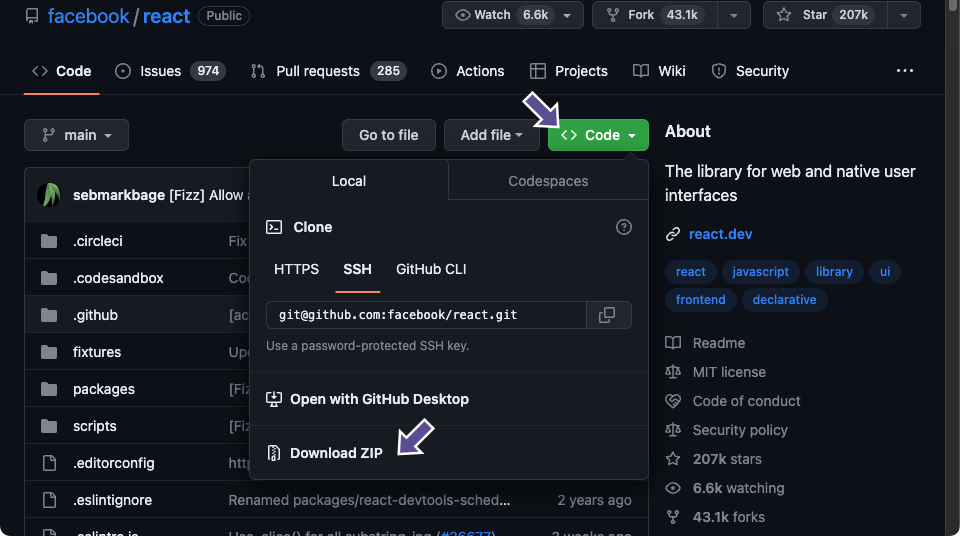
\includegraphics{images/image22.png}

Click on the green `Code' button, then the `Download ZIP' option. This
will download a single file, archived and compressed using the common
\href{https://en.wikipedia.org/wiki/ZIP_(file_format)}{ZIP} file format.
Double-clicking the file will extract its contents to a folder next to
the original .zip file.

An important distinction here is that you are downloading just the
codebase --- the files and folders of the repository --- and not the Git
repository itself. This means you lose some of the key functionality of
Git, for example, if the project maintainers make any updates to the
project, you will need to manually re-download the \texttt{.zip} file
and extract it again to see those changes, instead of being able to
easily pull these changes (more on this in the next example!).

\subsection{Clone}\label{sec-task2}

Another way to download a project to your computer is to use Git's
\texttt{clone} method. To use \texttt{clone}, we need to tell Git
installed on our computer to make a copy (or `clone') of another
repository, in this case from GitHub.

\subsection{Command-line}

First, we need to copy the address of the repository we want to clone.

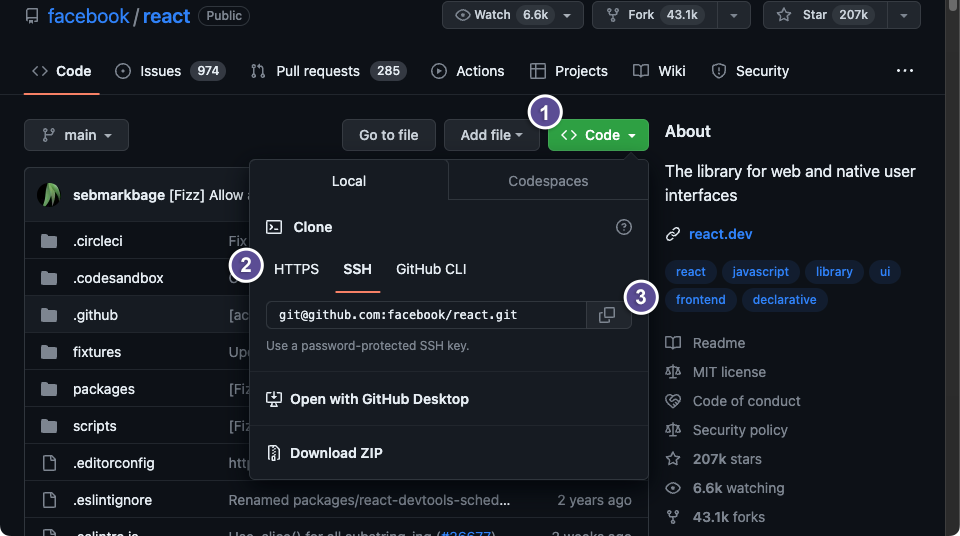
\includegraphics{images/image23.png}

\begin{enumerate}
\def\labelenumi{\arabic{enumi}.}
\item
  Click on the green button labelled ``Code''
\item
  Choose either HTTPS or SSH, depending on how you connect to GitHub
  with Git on your computer (see the Configuration section of Unit 1)
\item
  Copy the address
\end{enumerate}

Then in your terminal, navigate to your desired folder and issue the
following command:

\begin{Shaded}
\begin{Highlighting}[]
\NormalTok{git clone }\SpecialCharTok{\textless{}}\NormalTok{address}\SpecialCharTok{\textgreater{}}
\end{Highlighting}
\end{Shaded}

You should now see the repository has been cloned to your computer.

\subsection{GitHub Desktop}

First, navigate to the repository you want to clone on the GitHub
website.

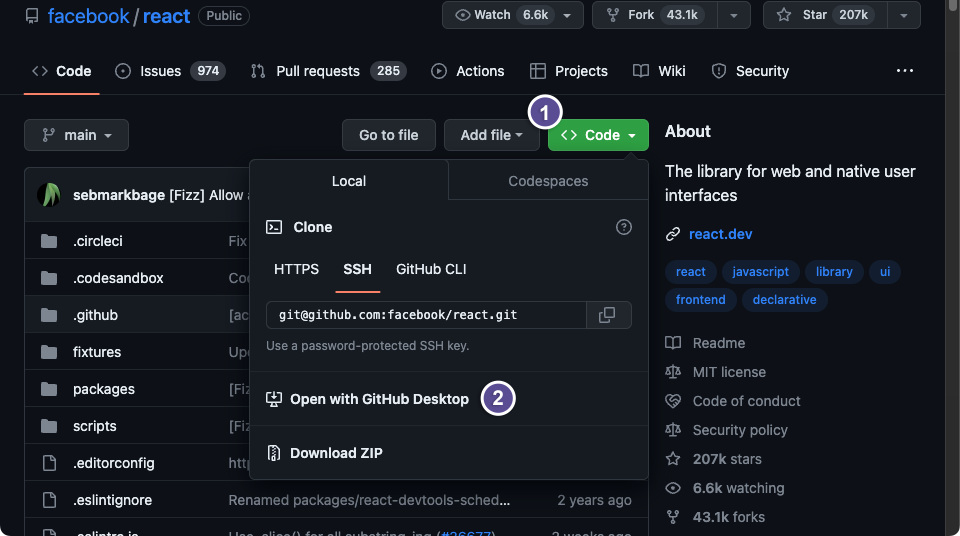
\includegraphics{images/image24.png}

\begin{enumerate}
\def\labelenumi{\arabic{enumi}.}
\item
  Click on the green button labelled `Code'
\item
  Click on `Open with GitHub Desktop'
\item
  You should then see a window like this pop up in GitHub Desktop:
\end{enumerate}

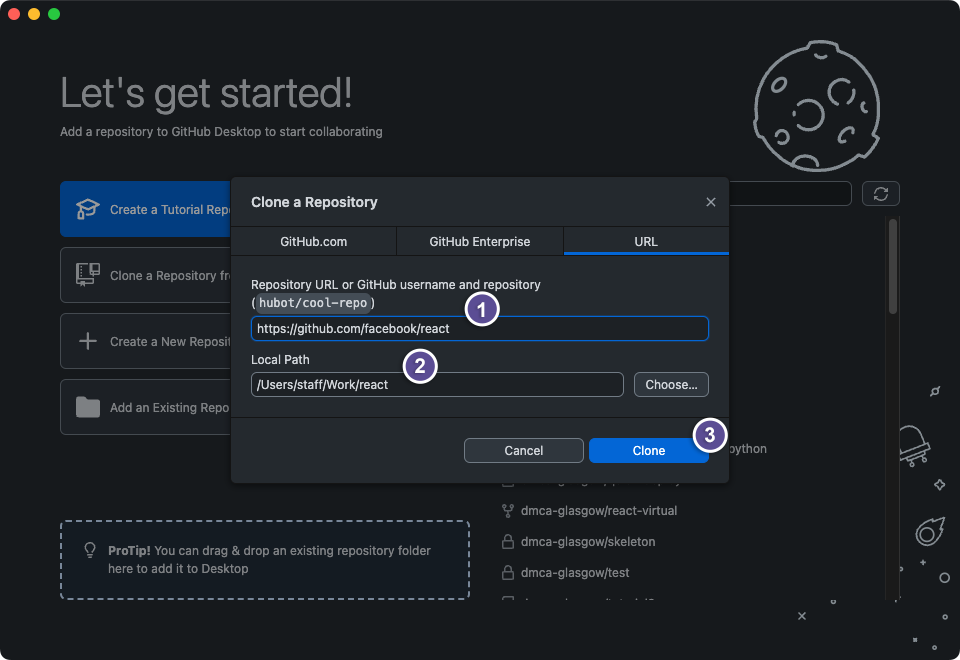
\includegraphics{images/image25.png}

\begin{enumerate}
\def\labelenumi{\arabic{enumi}.}
\item
  The URL of the repository on GitHub has automatically been populated
\item
  Choose where you would like the repository to be cloned to on your
  computer
\item
  Click `Clone'
\end{enumerate}

Using this approach, we have a copy of the files and folders in the
repository, but we have also copied the metadata which makes this into a
Git repository. To answer the example above, now if a project maintainer
makes an update to the project on GitHub, we can easily sync both
versions:

\subsection{Command-line}

In the project folder just issue the \texttt{pull} command:

\begin{Shaded}
\begin{Highlighting}[]
\NormalTok{git pull}
\end{Highlighting}
\end{Shaded}

\subsection{GitHub Desktop}

On GitHub Desktop, click the `Fetch origin' button in the top bar:

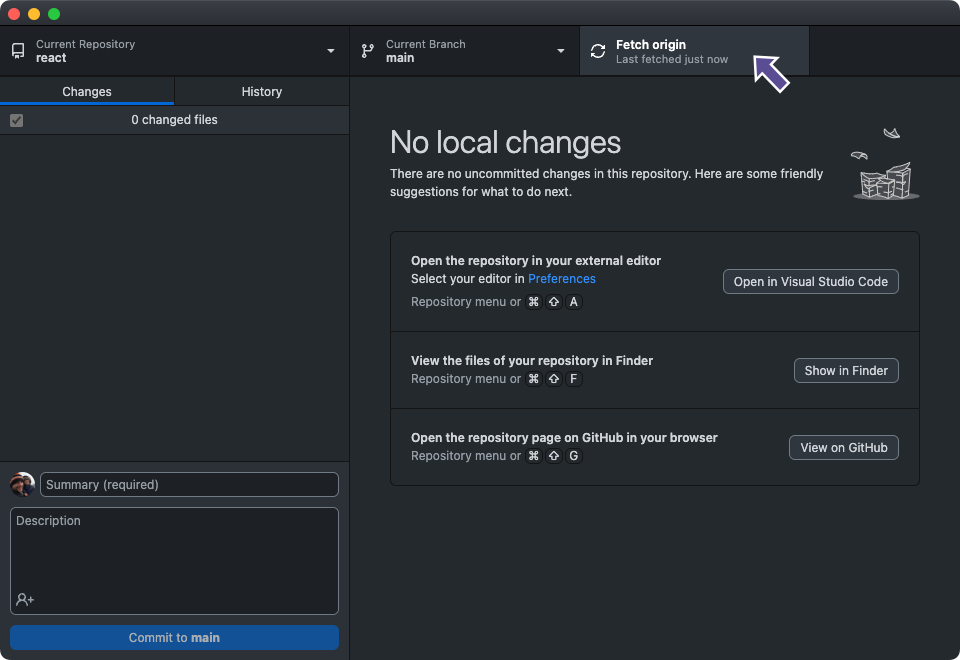
\includegraphics{images/image26.png}

\subsection{Create a new GitHub repository for your group
project}\label{create-a-new-github-repository-for-your-group-project}

To create a new GitHub repository we can either:

\begin{enumerate}
\def\labelenumi{\arabic{enumi}.}
\tightlist
\item
  Create a local repo and the push it (see
  \href{index.qmd\#sec-local_git}{notes})
\item
  Create a repo and GitHub and the clone it as we did on
  Task~\ref{sec-task2}.
\end{enumerate}

Lets look at the second approach. First, navigate to you GitHub profile
and click on \texttt{Repositories}. Then click on \texttt{New} :

\begin{center}
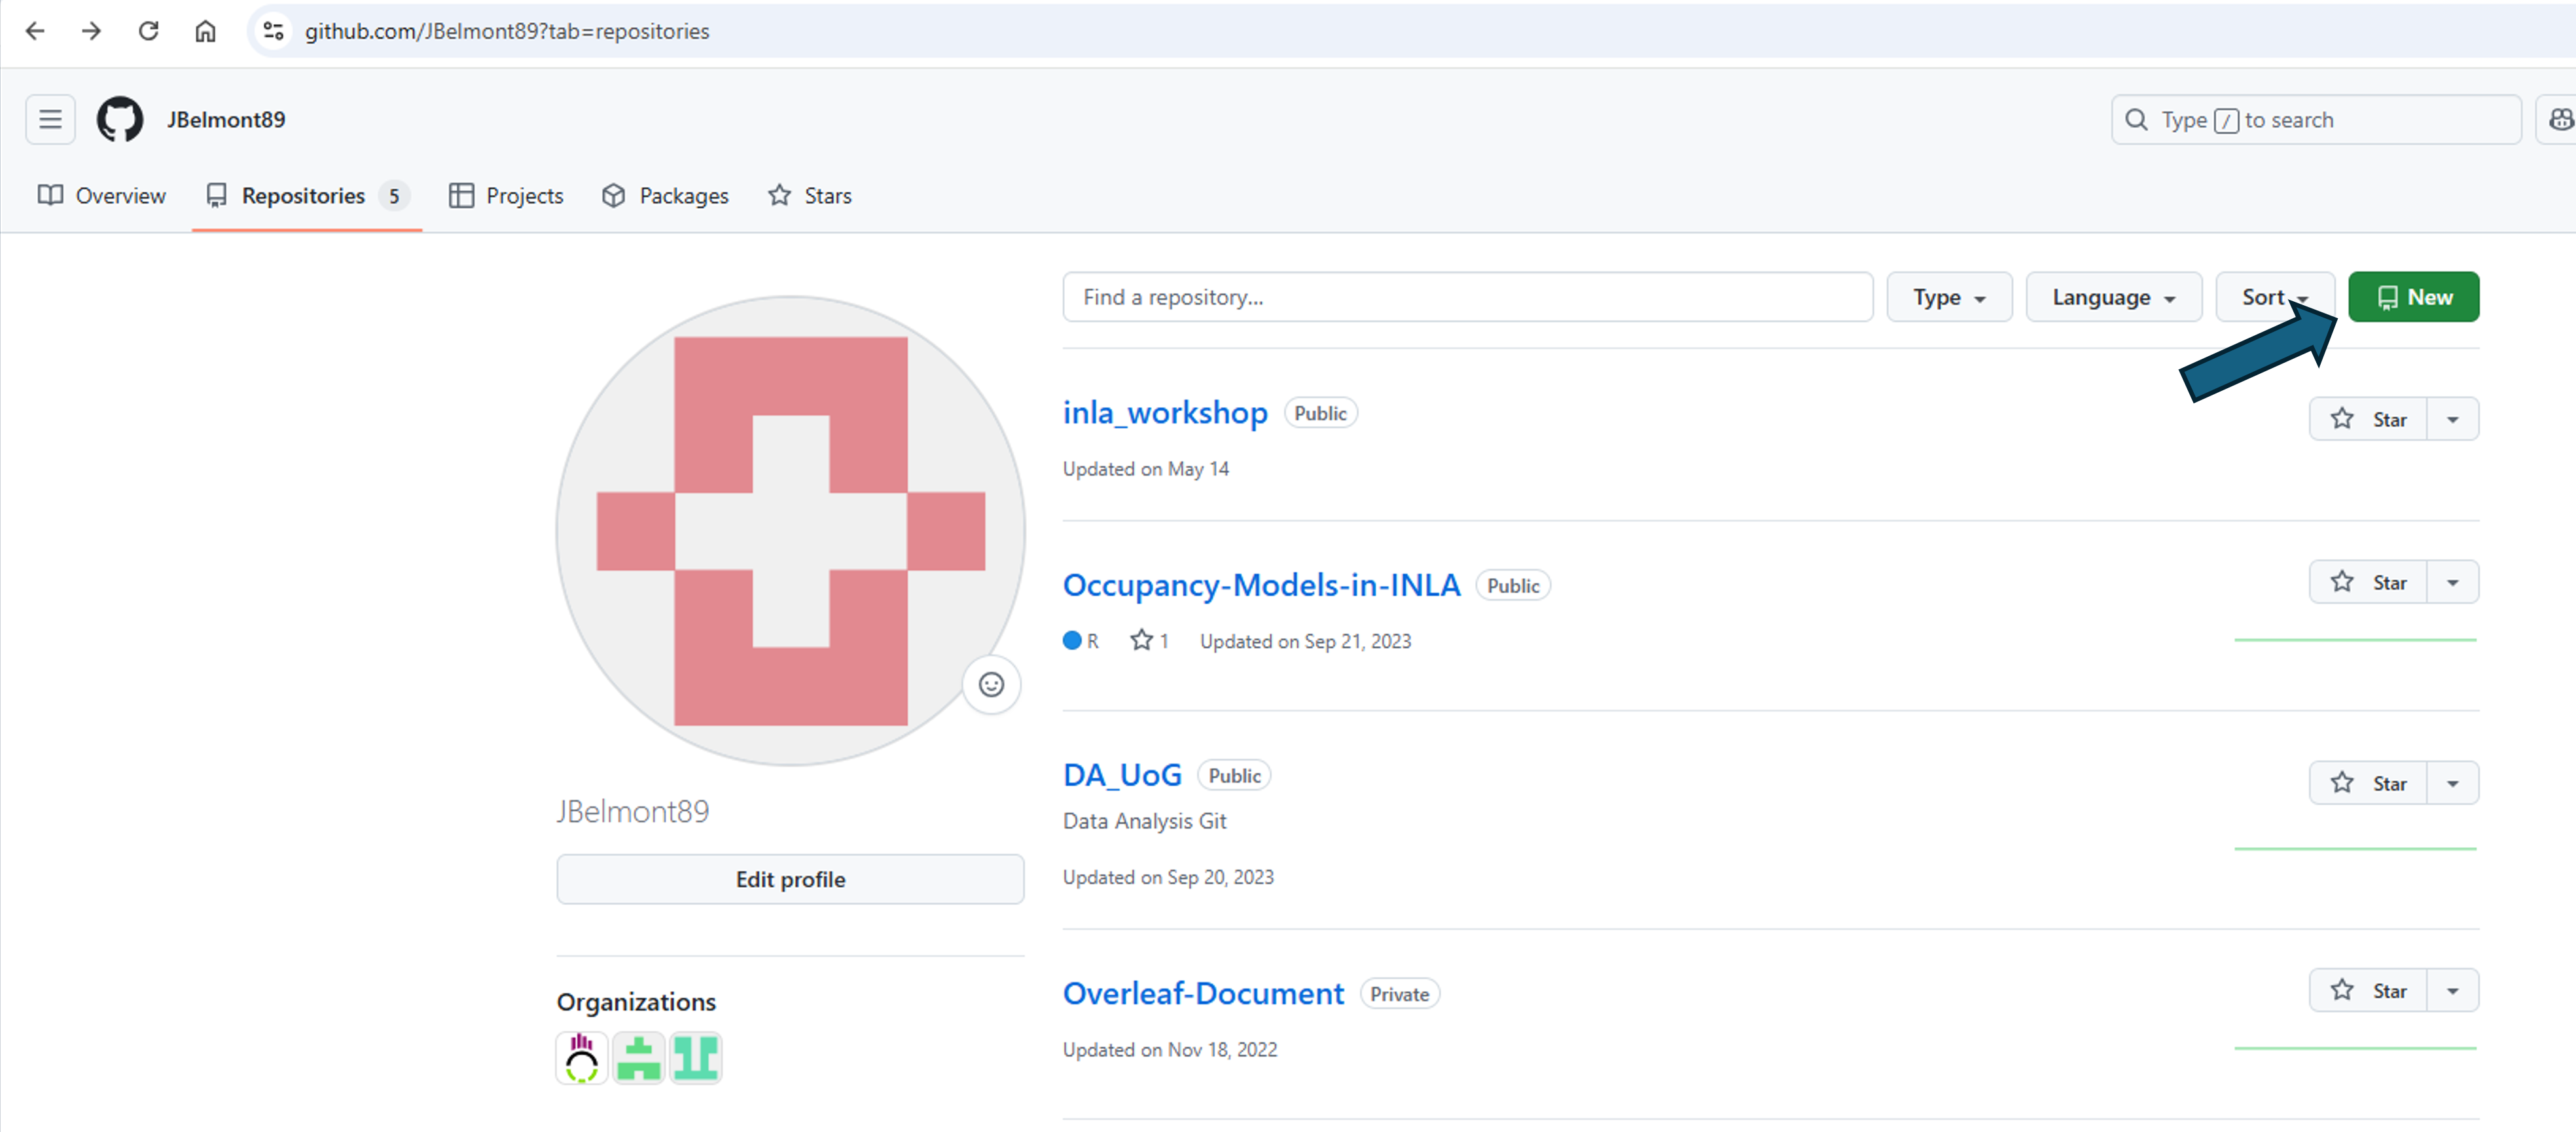
\includegraphics[width=5.91667in,height=\textheight]{images/git_new.png}
\end{center}

Then add a sensible name for your repo and configure it:

\begin{center}
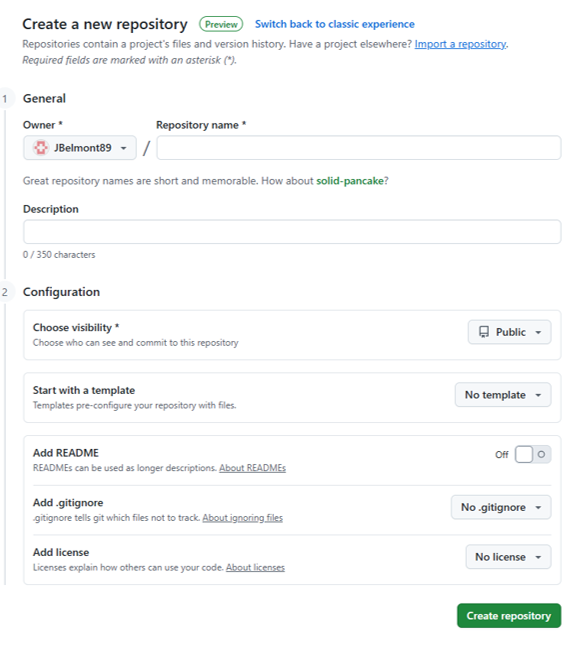
\includegraphics[width=4.91667in,height=\textheight]{images/git_new2.png}
\end{center}

Once you have created this repo you can clone it to your local machine
(see Task~\ref{sec-task2}).



\end{document}
